Because clojure is a dynamic language and a lisp it is usual to test the system
while writing the functions by using the REPL. In the case of this project this
was not enough because each component in the system was large and interconnected
to itself. Because of this I wrote tests covering each section.

\section{Parser - 320 assertions}
\label{section:parser-testing}
This component was the section that I focused most of my time testing on. This
is due to the fact that it is the only component that interfaces with input from
the user, user input can be of any form so it is effective to spend more effort
on places in the code that have to deal with it.

Because when I was developing the parser I had documentation that explained in
detail the domain language (see \cite{Ilghami2006}), it is was easy to test that
each of the different expressions worked as it was supposed to. Also, due to the
recursive nature of the language, I could test each expression individually to
check that it was working properly and then trust for the tests following it
that that expression would parse as expected.


\section{Pre-compiler - 147 assertions}
\label{section:pre-compiler-testing}
As I did not expect the parser to handle every case perfectly the next most
important place to test was the pre-compiler. This ended up being very useful as
a few errors did make it past the parser that I had not found. These errors
usually ended up being me misunderstanding how the clojure.spec library worked
and so I will not go into them here.

It was also useful to test that the data structures had the correct types of
children attached to them and that each of the properties attached to the data
structure was correctly filled.

\section{Encoder - 37 assertions}
\label{section:encoder-testing}
The encoder was the last component in the core that I built, and so it the
component that I spent the least time testing. What is important about testing
this component though is that this is the first time that a full end-to-end test
could be done. Because of this most of the tests in this section are tautologies
as most expressions are not expected to change too much as they pass through the
system.

\section{End to End test}
\label{section:end-to-end}
As a final test for the system I put together a simple example of a house with
several light in it. In this example the user has setup two rules: if it's the
afternoon and any of the lights are on then turn off all the lights; and if it's
either the morning or the evening and any of the lights are off then turn all
the lights on. This example is included in the `example/' directory in the base
of the source-code folder as well as in appendix \ref{appendix:home-example}.

The example is made up of several files, the problem file `p.prob' contains
information about the current state of the system, i.e. there are several
lights, some of them are on and some are not, and the hour of the day is 12.
There are three domain files the first of note is the `user-rules.dext' file,
this file is expected to be automatically generated by a user interface that the
manager of the automation system would configure.

The second file to look at would be the `time.dext' file, this extension is an
example of added functionality that could be provided by middleware as it
provides a series of axioms that use the `hour' predicate to provided a more
useful measure of time.

The third and final file is `light1.dext' which is the domain extension written
as a `driver' for the lights in the house. It is expected that this file would
be written by a third party and imported as part of a `plugin' package. This
file defines a series of operators which define the actions that the device as
well as the plugin can perform.

The results of this test is that a plan is formed to turn off all the lights as
the `afternoon' predicate is true and some of the lights are on, if the hour is
changed in the problem description file then the outcome of the test changes.
This the expected outcome of the test and shows that multiple domain extensions
can be combined together to perform a single task.

\begin{figure}
  \centering
  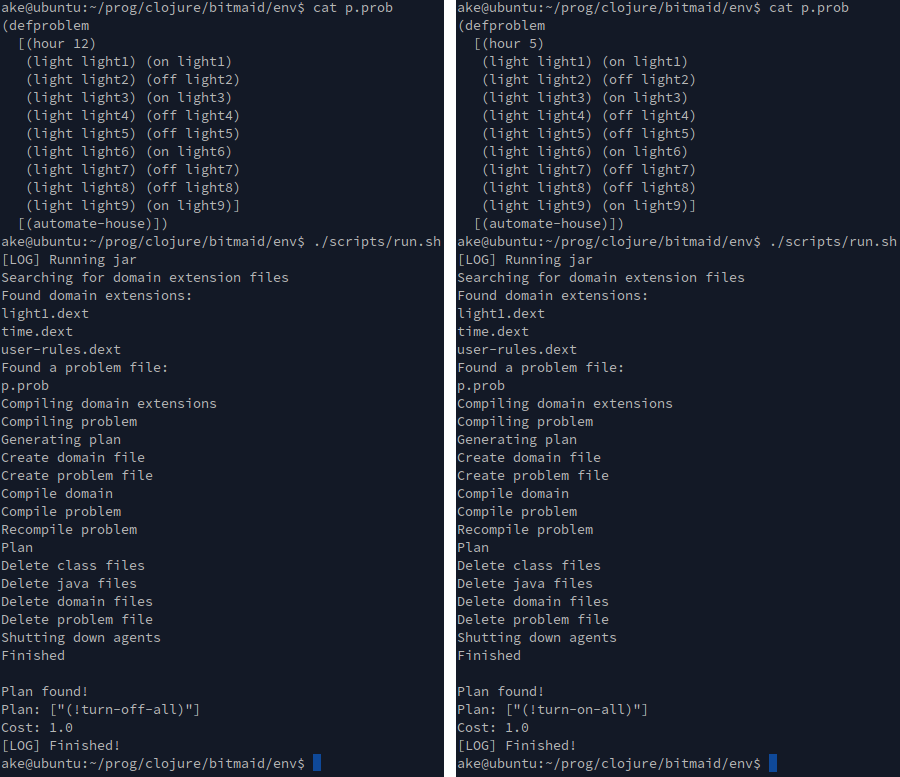
\includegraphics[width=1\linewidth]{figures/house-example.png}
  \caption{An example run of a simple example (a) with the hour set to 12 and
    (b) with the hour set to 5.}
  \label{fig:house-example}
\end{figure}

%%% Local Variables:
%%% mode: latex
%%% TeX-master: "../diss"
%%% End: